\chapter{Giới thiệu}
\label{chap:intro}

\section{Động lực nghiên cứu}
Bệnh Alzheimer (Alzheimer's disease -- AD) hiện là nguyên nhân hàng đầu dẫn đến hội chứng sa sút trí tuệ trên toàn cầu, làm suy giảm dần trí nhớ, năng lực tư duy cùng khả năng tự chủ trong sinh hoạt hằng ngày \cite{cdc2024alzheimers}. Trước khi chuyển biến thành sa sút trí tuệ thực thụ, phần lớn người bệnh trải qua một giai đoạn trung gian then chốt gọi là \emph{suy giảm nhận thức nhẹ} (Mild Cognitive Impairment -- MCI): tại giai đoạn này, trí nhớ hoặc một số chức năng nhận thức đã giảm sút rõ rệt so với mức bình thường của lứa tuổi, song họ vẫn duy trì được phần lớn các hoạt động sinh hoạt cơ bản và chỉ gặp trở ngại ở các công việc đòi hỏi tư duy phức tạp \cite{jack2018niaaa}. Đáng chú ý, diễn biến lâm sàng của nhóm đối tượng MCI lại rất đa dạng và không đồng nhất: có người nhanh chóng tiến triển sang sa sút trí tuệ chỉ sau một thời gian ngắn, nhưng cũng có người duy trì trạng thái ổn định suốt nhiều năm hoặc thậm chí có dấu hiệu cải thiện nhận thức \cite{petersen2018mci}. Xuất phát từ thực tế lâm sàng đó, khóa luận hướng tới giải quyết câu hỏi nghiên cứu cốt lõi: \emph{Dựa trên lịch sử thăm khám dọc của một người mắc MCI, liệu chúng ta có thể xếp hạng chính xác nguy cơ tiến triển sớm hay muộn của người đó hay không?}

Để trả lời thấu đáo câu hỏi này, việc chỉ quan sát người bệnh tại một thời điểm cắt ngang đơn lẻ là chưa đủ. Thật vậy, một ảnh chụp cộng hưởng từ não bộ (MRI) đơn thời điểm chỉ phản ánh trạng thái hình thái giải phẫu ở đúng ngày chụp, tương tự như một bức ảnh tĩnh khó lòng biểu thị được tốc độ và xu hướng biến đổi của cấu trúc mô. Trái lại, khi theo dõi chuỗi ảnh chụp lặp lại của cùng một cá thể qua thời gian, mô hình mới có đầy đủ cơ sở để nắm bắt tốc độ thoái hóa giải phẫu, tiêu biểu như tốc độ teo vùng hồi hải mã \cite{dong2021deepatrophy}. Đáng chú ý, trong dữ liệu theo dõi thực tế, khoảng cách giữa các lần khám không hề cố định mà biến thiên linh hoạt theo từng người bệnh (Bảng~\ref{tab:baseline-characteristics}). Do đó, tôi sử dụng mạng bộ nhớ dài ngắn hạn có xét thời gian (T-LSTM), cho phép tích hợp trực tiếp khoảng biến thiên thời gian thực tế giữa các lần khám vào quá trình cập nhật trạng thái ẩn của chuỗi \cite{baytas2017patient}.

Hơn nữa, tại mỗi lần thăm khám, khóa luận không chỉ dựa vào ảnh MRI đơn lẻ mà chủ động khai thác đồng thời ba nguồn thông tin mang tính bổ trợ sâu sắc:
\begin{enumerate}
\item \emph{Ảnh cộng hưởng từ cấu trúc 3D (MRI)}: cung cấp thông tin giải phẫu toàn diện của não bộ và ghi nhận các biến đổi vĩ mô quan trọng như teo hồi hải mã hay giãn rộng não thất \cite{weiner2015impact}.
\item \emph{Đặc trưng radiomics}: tập hợp các chỉ số toán học định lượng đo đạc trực tiếp hình dạng, phân bố cường độ sáng và độ thô mịn của kết cấu mô não trích xuất từ chính ảnh MRI \cite{vangriethuysen2017computational}.
\item \emph{Dữ liệu lâm sàng}: kết quả định lượng từ bài kiểm tra nhận thức tổng quát MMSE và thang đánh giá mức độ suy giảm chức năng sinh hoạt CDR \cite{folstein1975mmse,morris1993cdr}.
\end{enumerate}

Mặc dù cùng phản ánh tình trạng bệnh lý của một cá thể dưới các góc nhìn bổ trợ nhau, ba nguồn dữ liệu trên lại khác biệt sâu sắc về bản chất vật lý, số chiều biểu diễn và mức độ nhiễu tín hiệu. Vì vậy, phương thức kết hợp chúng đóng vai trò quyết định đối với chất lượng dự báo của mô hình. Điển hình trong nghiên cứu làm cơ sở tham chiếu trực tiếp cho khóa luận, Aghajanian và cộng sự (2025) đã sử dụng mạng tích chập (CNN), phân tích thành phần chính (PCA), T-LSTM và cơ chế chú ý (attention) trên chuỗi MRI dọc để ước lượng nguy cơ theo mô hình sống còn Cox \cite{aghajanian2025longitudinal}. Tuy nhiên, ở đúng cấu hình T-LSTM có attention (Bảng~2 của bài báo), khi ghép thêm đặc trưng radiomics chất xám vào đặc trưng CNN, chỉ số xếp hạng C-index trung bình lại giảm nhẹ từ 0.85 xuống 0.84 trên tập xác thực và từ 0.91 xuống 0.90 trên tập kiểm tra; vì lý do đó, các tác giả đã quyết định loại bỏ radiomics ở mô hình cuối cùng \cite{aghajanian2025longitudinal}. Kết quả thực nghiệm này đặt ra một câu hỏi khoa học gợi mở: \emph{Phải chăng việc radiomics chưa mang lại hiệu quả bổ sung là do cách thức ghép nối đặc trưng đơn giản chưa đủ năng lực khai thác các mối liên hệ chéo giữa các phương thức dữ liệu?}

Để giải quyết vấn đề đó, khóa luận kế thừa bài toán tiên lượng cùng khung dữ liệu tham chiếu của Aghajanian và cộng sự, song tập trung tái thiết kế phương thức hợp nhất ba nguồn thông tin. Thay vì chỉ ghép nối đơn thuần các vectơ đặc trưng nằm cạnh nhau, tôi tiến hành mô hình hóa tường minh tương tác song tuyến giữa từng cặp nguồn. Cụ thể, với ba nguồn MRI (M), radiomics (R) và lâm sàng (C), ta có ba cặp tương tác khả dĩ: MRI--Radiomics (MR), MRI--Lâm sàng (MC) và Radiomics--Lâm sàng (RC). Nhằm khắc phục triệt để nguy cơ bùng nổ tham số khi thực hiện nhân chéo trên cỡ mẫu y tế hạn chế, mỗi lớp tương tác song tuyến được nén chặt bằng \emph{phân rã tensor Canonical Polyadic (CP) hạng thấp} \cite{kolda2009tensor,liu2018lowrank}, sau đó truyền ngược lại biểu diễn gốc thông qua kết nối phần dư có cổng điều tiết động. Đặc biệt, xuất phát từ thực tế radiomics vốn được trích xuất từ chính ảnh MRI, tôi đề xuất kiến trúc tinh giản mang tên \textbf{RC-Free Pairwise Fusion (RC-Free)}: lấy MRI làm nút trung tâm kết nối cho hai cặp MR và MC, đồng thời chủ động loại bỏ tương tác trực tiếp RC. Tính đúng đắn và hiệu quả của lựa chọn kiến trúc này được kiểm chứng sáng tỏ qua thực nghiệm đối chứng với toàn bộ bảy cấu hình tương tác cặp ở Mục~\ref{sec:new-topology}.

\section{Phát biểu bài toán}
Khóa luận giải quyết bài toán xây dựng mô hình học sâu xếp hạng nguy cơ tiến triển cho nhóm đối tượng mắc MCI dựa trên bộ dữ liệu của Sáng kiến Hình ảnh Thần kinh Bệnh Alzheimer (ADNI) \cite{weiner2015impact}. Quần thể nghiên cứu gồm 359 người tham gia có đủ ba lần chụp MRI trong vòng 18 tháng kể từ lần khám ban đầu; mỗi lần chụp đều được liên kết đồng bộ với bộ đặc trưng radiomics và điểm lâm sàng tương ứng. Ba mốc thời gian chụp $s_1<s_2<s_3=p\leq L$ tạo thành một chuỗi quan sát dọc có khoảng cách thời gian biến thiên theo từng người bệnh. Dựa trên chuỗi ba lần khám này, phương pháp đề xuất ước lượng cho mỗi cá thể một chỉ số log-nguy cơ $\eta_i\in\mathbb R$ để xếp hạng rủi ro suy giảm nhận thức trong tương lai: người có điểm $\eta_i$ càng cao thì được dự báo có nguy cơ tiến triển thành bệnh càng sớm.

\begin{figure}[H]
\centering
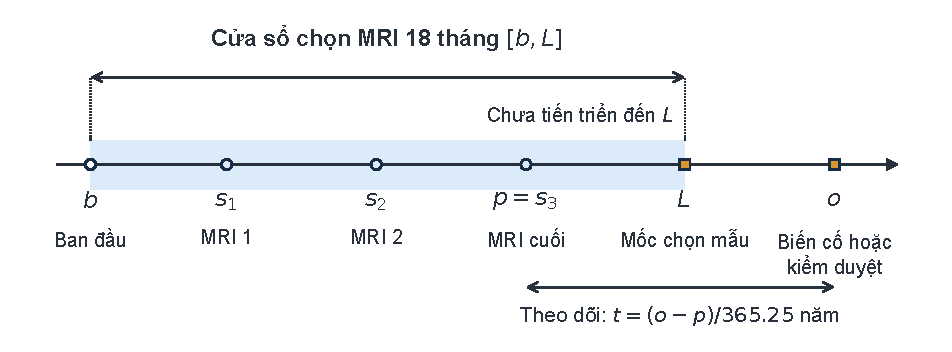
\includegraphics[width=\textwidth]{image/mci-progression-timeline.pdf}
\caption{Bài toán dự đoán tiến triển MCI theo thời gian}
\label{fig:problem-timeline}
\end{figure}

Hình~\ref{fig:problem-timeline} minh họa trực quan trục thời gian của bài toán, phân định rành mạch giữa giai đoạn quan sát đầu vào (ba lần chụp trước mốc chọn mẫu $L$, được xác định bằng ngày khám ban đầu cộng 18 tháng lịch) và giai đoạn theo dõi kết cục lâm sàng sau mốc $L$. Để lượng hóa chính xác mức độ suy giảm nhận thức cũng như chức năng sinh hoạt, khóa luận sử dụng hai thang đo chuẩn mực trong y khoa:
\begin{enumerate}
\item \emph{MMSE (Mini-Mental State Examination)}: thang điểm từ 0 đến 30 đánh giá toàn diện năng lực nhận thức tổng quát; điểm số càng suy giảm phản ánh mức độ sa sút nhận thức càng nghiêm trọng \cite{folstein1975mmse}.
\item \emph{CDR-global (Clinical Dementia Rating toàn cục)}: phân loại mức độ sa sút trí tuệ thành năm bậc gồm 0 (bình thường), 0.5 (sa sút trí tuệ rất nhẹ), 1 (nhẹ), 2 (vừa) và 3 (nặng) theo hướng dẫn chấm điểm chuẩn hóa \cite{morris1993cdr,knightcdrscoring}.
\end{enumerate}

Kế thừa quy ước lâm sàng của Aghajanian và cộng sự \cite{aghajanian2025longitudinal}, trong nghiên cứu này, \emph{biến cố tiến triển} được ghi nhận tại lần thăm khám đầu tiên sau mốc $L$ thỏa mãn điều kiện có điểm MMSE $<24$ hoặc CDR-global $\geq1$. Đây là biến cố định nghĩa theo ngưỡng suy giảm chức năng nhận thức. Trong quá trình theo dõi dọc dài hạn, nhiều người tham gia rời khỏi nghiên cứu hoặc thời gian dự án kết thúc khi họ chưa từng vượt qua ngưỡng này; do đó, trạng thái bệnh lý sau này của họ không thể biết trước, ngoại trừ sự thật là họ vẫn duy trì trạng thái ổn định cho đến lần khám cuối cùng. Hiện tượng thống kê này được gọi là \emph{kiểm duyệt phải} (right-censoring). Thay vì ép bài toán thành phân loại nhị phân Có/Không (vốn buộc phải gán nhãn sai lệch hoặc loại bỏ các ca kiểm duyệt), khóa luận thiết lập bài toán trong khung \emph{phân tích sống còn} nhằm tận dụng tối đa và công bằng cả thông tin kiểm duyệt lẫn độ dài thời gian theo dõi thực tế.

Bên cạnh đó, về mặt phương pháp luận, cần lưu ý một điểm then chốt trong cách tính trục thời gian: mô hình tính thời gian sống còn bắt đầu từ ngày chụp MRI lần ba $p$, trong khi điều kiện chọn mẫu lại đòi hỏi người bệnh phải duy trì trạng thái ổn định cho đến hết mốc 18 tháng $L$. Khi $p<L$, khoảng thời gian từ $p$ đến $L$ chắc chắn không xảy ra biến cố do chính quy tắc chọn mẫu quy định, tạo nên hiện tượng \emph{sai lệch thời gian bất tử} \cite{suissa2008immortal} nếu áp dụng mô hình như một công cụ dự báo trực tiếp ngay tại thời điểm chụp $p$. Do vậy, các kết quả trong khóa luận được diễn giải một cách cẩn trọng cho bài toán xếp hạng hồi cứu trên nhóm đối tượng đã xác định là duy trì ổn định đến mốc $L$ (phân tích chi tiết tại Mục~\ref{sec:study-design} và Mục~\ref{sec:study-limitations}).

\section{Thách thức và phạm vi nghiên cứu}
Quá trình xây dựng mô hình học sâu sống còn đa phương thức trên chuỗi dữ liệu y tế dọc đặt ra ba thách thức kỹ thuật trọng tâm:
\begin{enumerate}
\item \emph{Cân bằng giữa năng lực biểu diễn tương tác và dung lượng tham số}: Phép ghép nối vectơ không làm tăng tham số tại bước kết hợp, song lại bỏ lỡ các tích chéo bậc hai giữa các nguồn. Ngược lại, phép tích ngoài bao quát trọn vẹn mọi tương tác song tuyến nhưng lại khiến số trọng số của lớp tuyến tính tiếp theo bùng nổ theo cấp số nhân \cite{zadeh2017tensor,liu2018lowrank}, rất dễ dẫn đến hiện tượng quá khớp trên tập huấn luyện chỉ có 251 người bệnh. Phân rã tensor CP cho phép nén mạnh số tham số nhờ cấu trúc hạng thấp \cite{kolda2009tensor,liu2018lowrank}, song mức độ đánh đổi giữa việc nén tham số và chất lượng phân tầng nguy cơ đòi hỏi phải được kiểm chứng thực nghiệm cẩn trọng.
\item \emph{Nguy cơ dư thừa biểu diễn giữa các cặp tương tác}: Do đặc trưng radiomics vốn được trích xuất từ chính ảnh MRI, trong khi điểm lâm sàng vừa là biến đầu vào vừa liên quan mật thiết đến tiêu chí biến cố, việc duy trì đồng thời cả ba cặp tương tác (MR, MC, RC) có thể làm cồng kềnh mô hình mà không cung cấp thêm lượng tin mới. Do đó, cần có một khảo sát thực nghiệm có hệ thống để xác định cấu trúc cặp tương tác tinh gọn và tối ưu nhất.
\item \emph{Huấn luyện xếp hạng sống còn trên chuỗi ảnh thể tích 3D dung lượng lớn}: Do mỗi người bệnh sở hữu tới ba khối ảnh não 3D chiếm dụng bộ nhớ GPU đáng kể, mỗi lượt huấn luyện chỉ có thể nạp vào một số lượng rất ít bệnh nhân. Mặt khác, để hàm mất mát Cox học được cách xếp hạng nguy cơ, mỗi lô dữ liệu bắt buộc phải chứa ít nhất một người gặp biến cố đứng cạnh những người ổn định lâu hơn; nếu chia lô ngẫu nhiên thuần túy, nhiều lô huấn luyện sẽ không có ca biến cố nào để cập nhật trọng số.
\end{enumerate}

Để vượt qua các thách thức trên, trong khuôn khổ khóa luận, tôi tiến hành khảo sát có kiểm soát ba lựa chọn thiết kế kiến trúc. Thứ nhất là đối chiếu tường minh giữa phương thức ghép nối truyền thống và tích ngoài song tuyến. Thứ hai là lượng hóa mức độ cắt giảm tham số và sự đánh đổi hiệu năng khi áp dụng phân rã tensor CP. Thứ ba là kiểm nghiệm toàn diện bảy cấu hình tương tác cặp nhằm chứng minh tính ưu việt của kiến trúc RC-Free đề xuất. Mọi thực nghiệm cốt lõi đều được thực hiện trên cùng một cách chia tập dữ liệu cố định theo người tham gia và lặp lại qua ba lần khởi tạo ngẫu nhiên độc lập (seed). Hiệu năng của các phương pháp được đo lường khách quan bằng ba thước đo sống còn bổ trợ: chỉ số đồng thuận Harrell's C-index, diện tích dưới đường cong ROC phụ thuộc thời gian có trọng số kiểm duyệt (IPCW-ROC) và đường cong sống còn Kaplan--Meier.

\section{Câu hỏi nghiên cứu}
Để dẫn dắt các thực nghiệm ở Chương~\ref{chap:results} theo một mạch lập luận khoa học chặt chẽ, tôi cụ thể hóa mục tiêu nghiên cứu thành năm câu hỏi nghiên cứu (RQ1--RQ5), được tổng hợp trong Bảng~\ref{tab:rq}. Trong đó, hai câu hỏi đầu tiên đánh giá giá trị thông tin của dữ liệu dọc và đóng góp bổ trợ từ radiomics cùng điểm lâm sàng; RQ3 đối chứng trực tiếp giữa phép ghép nối và tương tác tích ngoài; cuối cùng, RQ4 và RQ5 phân tích sâu hiệu quả nén tham số của phân rã CP và tính ưu việt của kiến trúc tinh giản RC-Free.

\begin{table}[H]
\centering\small
\caption[Các câu hỏi nghiên cứu và phương pháp kiểm chứng]{Các câu hỏi nghiên cứu và phương pháp kiểm chứng.}
\label{tab:rq}
\setlength{\tabcolsep}{6pt}
\renewcommand{\arraystretch}{1.12}
\begin{tabularx}{\textwidth}{@{}Y Y@{}}
\toprule
\textbf{Câu hỏi nghiên cứu} & \textbf{Phương pháp kiểm chứng} \\
\midrule
\textbf{RQ1.} MRI ở nhiều thời điểm có mang lại khả năng phân biệt nguy cơ cao hơn so với chỉ dùng MRI cuối cùng không? & Đối chiếu mô hình \textit{MRI cuối} với \textit{MRI dọc và T-LSTM} cùng \textit{MRI dọc, T-LSTM và attention} để khảo sát vai trò của thông tin theo thời gian. \\
\addlinespace
\textbf{RQ2.} Bổ sung radiomics và lâm sàng có cải thiện khả năng phân biệt nguy cơ so với chỉ dùng MRI không? & Đối chiếu \textit{MRI dọc, T-LSTM và attention} với \textit{Ghép nối ba nguồn} sử dụng đồng thời MRI, radiomics và lâm sàng. \\
\addlinespace
\textbf{RQ3.} Tương tác theo cặp có hiệu quả hơn ghép nối đặc trưng không? & So sánh ghép nối và tích ngoài qua ba lần chạy, giữ cùng cách huấn luyện và cùng trọng số khởi tạo cho các phần chung. \\
\addlinespace
\textbf{RQ4.} Phân rã CP giảm bao nhiêu tham số của lớp tương tác và ảnh hưởng thế nào đến C-index? & So sánh Full Outer-Product và Full CP về số tham số ở từng phạm vi và C-index xác thực qua ba lần chạy. \\
\addlinespace
\textbf{RQ5.} Có thể bỏ bớt một số cặp tương tác mà vẫn duy trì khả năng phân biệt nguy cơ không? & Đối chiếu cả bảy cấu trúc CP có ít nhất một cặp tương tác (các cấu hình 1 cặp, 2 cặp như RC-Free, MR-Free, MC-Free và Full CP). \\
\bottomrule
\end{tabularx}
\end{table}

\FloatBarrier
\Needspace{10\baselineskip}
\section{Đóng góp của khóa luận}
Khóa luận mang lại ba đóng góp chính cả về mặt phương pháp luận lẫn thực nghiệm:
\begin{enumerate}
\item \emph{Quy trình học sâu sống còn đa phương thức toàn diện trên dữ liệu dọc}: Khóa luận tích hợp đồng bộ ảnh MRI 3D (mã hóa qua ResNet-18 3D khởi tạo từ MedicalNet \cite{chen2019med3d}), đặc trưng radiomics toàn não và các chỉ số lâm sàng MMSE/CDR qua ba lần khám liên tiếp, kết hợp hài hòa với T-LSTM \cite{baytas2017patient}, cơ chế attention và mô hình Cox để ước lượng chính xác nguy cơ tiến triển.
\item \emph{Cơ chế hợp nhất cặp CP có cổng điều tiết và cấu trúc tinh gọn RC-Free}: Khóa luận thay thế lớp tích ngoài đầy đủ bằng tham số hóa CP hạng thấp và truyền dẫn thông tin tương tác ngược về từng nguồn qua kết nối phần dư có cổng động. Bằng việc lấy MRI làm trung tâm kết nối cho hai cặp MR và MC, kiến trúc \textbf{RC-Free} loại bỏ thành công cặp tương tác RC mà vẫn duy trì trọn vẹn sự hiện diện của cả ba nguồn dữ liệu đầu vào.
\item \emph{Đánh giá thực nghiệm có kiểm soát về độ tinh giản tham số và năng lực phân tầng sống còn}: Phân rã CP giúp cắt giảm tới \textbf{98.38\%} số tham số ở ba lớp song tuyến đầu (Bảng~\ref{tab:interaction-parameters}), trong khi thiết kế RC-Free tiết kiệm thêm \textbf{15460 tham số} so với cấu trúc Full CP. Trên cùng một tập xác thực qua ba lần khởi tạo ngẫu nhiên, RC-Free xác lập C-index trung bình cao nhất trong toàn bộ bảy cấu hình tương tác cặp (\textbf{0.8347}, Bảng~\ref{tab:new-topology}), đồng thời phân tách rõ rệt hai nhóm nguy cơ trên đường cong Kaplan--Meier ($p=0.0134$ trên tập xác thực; $p<0.001$ trên tập kiểm tra hậu nghiệm, Bảng~\ref{tab:km-statistics}).
\end{enumerate}

Phần còn lại của khóa luận được tổ chức thành bốn chương tiếp nối nhau. Chương~\ref{chap:background} hệ thống hóa các khái niệm nền tảng về dữ liệu dọc, phân tích sống còn và điểm lại các công trình liên quan. Chương~\ref{chap:method} mô tả chi tiết quy trình xử lý dữ liệu, kiến trúc mô hình đề xuất RC-Free và khung đánh giá thực nghiệm. Chương~\ref{chap:results} lần lượt trình bày kết quả thực nghiệm giải đáp trọn vẹn từ RQ1 đến RQ5 cùng các phân tích sống còn chuyên sâu. Cuối cùng, Chương~\ref{chap:discussion} thảo luận các bài học rút ra, nêu rõ các giới hạn còn tồn tại, đề xuất hướng phát triển tiếp theo và đúc kết kết luận chung của khóa luận.
